\section{Preliminary Data Analysis}
In this section, the given data will be explored and visualised.

\subsubsection{Hazard Rate}
Before trying to find a policy to optimally schedule preventive maintenance, it would be useful to first consider whether maintenance is helpful at all. To do this, we can consider the hazard rate of the machine. An increasing hazard rate results in a decreased expected lifetime over time while a decreasing hazard rate results in an increased expected lifetime. Below, you see a plot of this.
\begin{figure}[H]
\centering
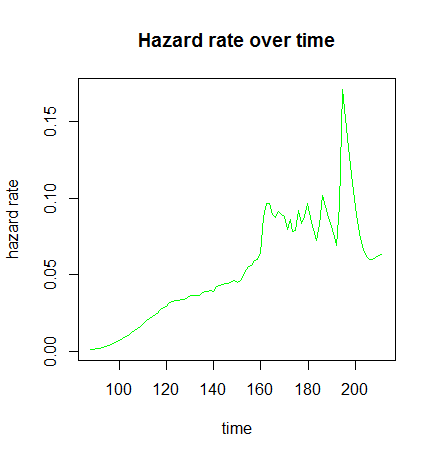
\includegraphics[width=0.8\textwidth]{Plots/HazardRate.png}
\caption{Hazard rate of the machine under consideration.}
\end{figure}
The hazard rate seems to be decrease after 200 hours, but this can be explained by the fact that there is only one trace that lasted over 200 hours. Hence, we can conclude that the hazard rate rises over time (at least for the first 200 hours). This means that repairing would increase the expected life time of the machine.

\subsection{Time Until Failure}
To be able to predict the remaining time until a failure, it is helpful to know how the total lifetime of the machine is distributed. In this section we will attempt to fit the lifetime to a distribution.

\subsubsection{Normality}
The first guess for a fitting distribution would be a normal distribution. However, the Shapiro-Wilk normality test rejected the hypothesis that the lifetimes are normally distributed with a p-value of $1.26\times 10^{-5}$. Hence, we can safely conclude that the data do not follow a normal distribution. This is also visible on the following quantile-quantile plot.
\begin{figure}[H]
\centering
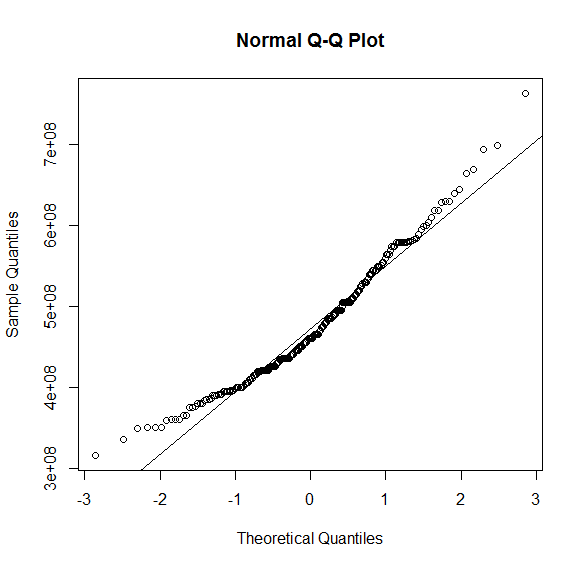
\includegraphics[width=0.8\textwidth]{Plots/QQPlot.png}
\caption{Quantile-quantile plot of the trace lifetimes.}
\end{figure}

\subsubsection{Cullen and Frey graph}
\begin{figure}[H]
\centering
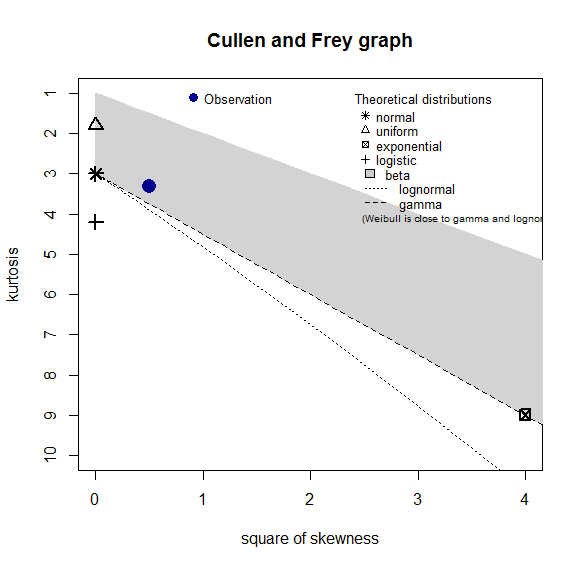
\includegraphics[width=0.8\textwidth]{Plots/CullenAndFray.png}
\caption{Cullen and Fray graph of the data.}
\end{figure}
Above, a Cullen and Fray graph is plotted. The data is placed based on its kurtosis and skewness. A few well-known distributions are also plotted on this plane. This plot would suggest a beta distribution. However, the beta distribution has a support of $[0,1]$ while the lifetime is not bounded. Other distributions that have similar kurtosis and skewness are the Weibull distribution and the gamma distribution.\\
After estimating the parameters for each of these distributions and performing a Anderson-Darling Goodness-of-Fit test, the gamma-distribution seems to fit the data best with a p-value of $0.195$ versus a $p$-value of $0.00444$. Below, a plot shows the density of this distribution plotted over the observed density. As you can see, it does not fit the data very well.
\begin{figure}[H]
\centering
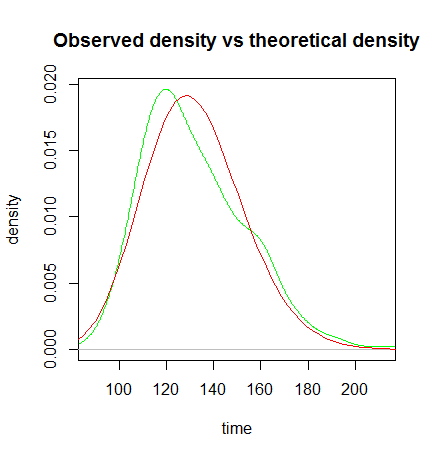
\includegraphics[width=0.8\textwidth]{Plots/LifetimeDensity.png}
\caption{The observed density plotted over the density of the Gamma distribution}
\end{figure}

\subsubsection{Phase-Type distribution}
As the class of Phase-Type distributions is dense in the space of positive continuous distributions, a Phase-Type distribution could also be used to model the lifetimes. However, Phase-Type distributions have a few disadvantages: The number of parameters grows quadratically with the amount of states and a lot of these parameters are redundant. Furthermore, convergence of the EM-algorithm (to estimate the parameters) is slow and can get stuck in saddle points and local maxima \cite{Asmussen1996}.

\subsubsection{Transition Times}
If we view each event as a state and view switching from one event to another as a transition. Then we could model the machine as a transitioning system. It would then be interesting to see how the transition times are distributed; whether they are of the same family of distributions and whether they are independent. \\
When using the Anderson-Darling Goodness-of-Fit test for testing whether the transition times are exponentially distributed, the resulting p-values are rather low. 